\chapter{Validation}
\label{ch:validation}
Nous désirons mesurer deux aspects de notre programme : la qualité des stratégies décrites dans le sujet de \ac{TP} et la complexité de chaque algorithme. Pour cela, nous avons mis en place un championnat qui oppose différentes configurations, ainsi que des mesures de complexité pour chaque algorithme. Les statistiques sont obtenues sur 100 itérations, sauf pour certaines profondeurs 6 pour des raisons de temps de calcul. Les résultats sont présentés dans les sections suivantes.


\section{Mesure de complexité : Exploration de l'arbre de jeu}
\label{sec:game_tree_exploration}
Nous comparons ici la complexité en temps et en nombre de nœuds explorés. Nous avons mesuré ces deux aspects sur 24 configurations. Elles correspondent à un affrontement entre soit Minimax, soit Alpha-Beta contre un joueur aléatoire avec une profondeur de recherche de 2, 4 et 6, sur différentes stratégies. Nous avons mesuré le temps de calcul pour chaque partie jouée. L'unité des valeurs entre parenthèses est la seconde.


\begin{table}[H]
    \centering
    \caption{Analyse comparative du temps d'exécution d'une partie en fonction des profondeurs et stratégies (rapport NegamaxAlphaBeta(gauche)/Negamax(droite))}
    \resizebox{0.9\textwidth}{!}{% Resize table to fit within the text width, keeping aspect ratio
        \begin{tabular}{
            @{}
            >{\raggedright\arraybackslash}p{1cm}
            >{\raggedright\arraybackslash}p{4cm}
            S
            S
            S
            @{}
            }
            \toprule
            \textbf{Depth} & \textbf{Strategy}           & {\textbf{Mean (\%)}}      & {\textbf{Std (\%)}}      \\
            \midrule
            \midrule
            \multirow{4}{*}{2}
                           & Positional                  & {74.10 (0.03 vs 0.04)}    & {198.71 (0.02 vs 0.01)}  \\
                           & Absolute                    & {86.94 (0.01 vs 0.02)}    & {208.26 (0.02 vs 0.01)}  \\
                           & Mobility                    & {54.55 (0.06 vs 0.12)}    & {83.37 (0.02 vs 0.03)}   \\
                           & Mixed (thresholds=[30, 55]) & {67.22 (0.06 vs 0.08)}    & {140.54 (0.04 vs 0.03)}  \\
            \midrule
            \multirow{4}{*}{4}
                           & Positional                  & {14.56 (0.90 vs 6.21)}    & {14.38 (0.30 vs 2.06)}   \\
                           & Absolute                    & {24.09 (0.51 vs 2.10)}    & {16.92 (0.19 vs 1.15)}   \\
                           & Mobility                    & {13.04 (1.50 vs 11.52)}   & {11.27 (0.49 vs 4.38)}   \\
                           & Mixed (thresholds=[30, 55]) & {15.93 (1.17 vs 7.34)}    & {12.67 (0.40 vs 3.18)}   \\
            \midrule
            \multirow{4}{*}{6}
                           & Positional                  & {8.45 (35.20 vs 416.65)}  & {2.60 (2.82 vs 108.49)}  \\
                           & Absolute                    & {12.23 (20.14 vs 164.64)} & {18.39 (13.95 vs 75.87)} \\
                           & Mobility                    & {2.83 (39.32 vs 1390.49)} & {1.03 (7.65 vs 745.69)}  \\
                           & Mixed (thresholds=[30, 55]) & {3.17 (17.34 vs 546.98)}  & {4.36 (5.04 vs 115.61)}  \\
            \bottomrule
        \end{tabular}
    }
\end{table}


\subsection{Nombre de nœuds explorés}
\label{subsec:node_explored}
Nous avons mesuré à chaque coup des joeurs, le nombre de nœuds explorés. Nous pouvons donc comparer chaque algorithme sur un graphe pour chaque profondeur donnée\footnote{Chaque figure est disponible séparément dans les appendices \ref{app:node_explored}.}. Nous avons également calculé le nombre moyen de nœuds explorés pour chaque configuration. Les résultats sont présentés dans les tableaux \ref{tab:node_explored_summary} et \ref{tab:node_explored_summary-2}.

\begin{figure}[H]
    \centering
    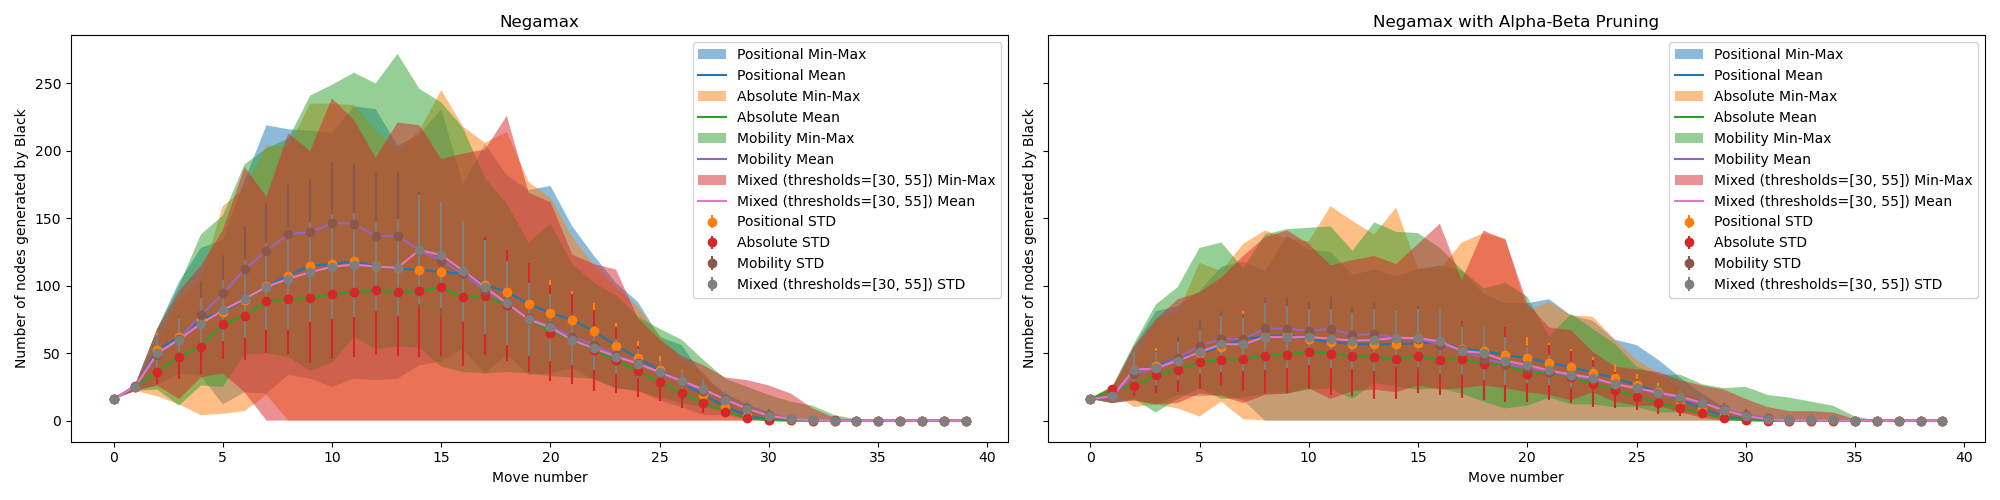
\includegraphics[width=\textwidth]{ressources/Number of nodes generated by Black_depth_2_combined.png}
    \caption{Nombre de nœuds explorés par Minimax et Alpha-Beta en profondeur 2.}
    \label{fig:complexity_node_explored-2}
\end{figure}

\begin{figure}[H]
    \centering
    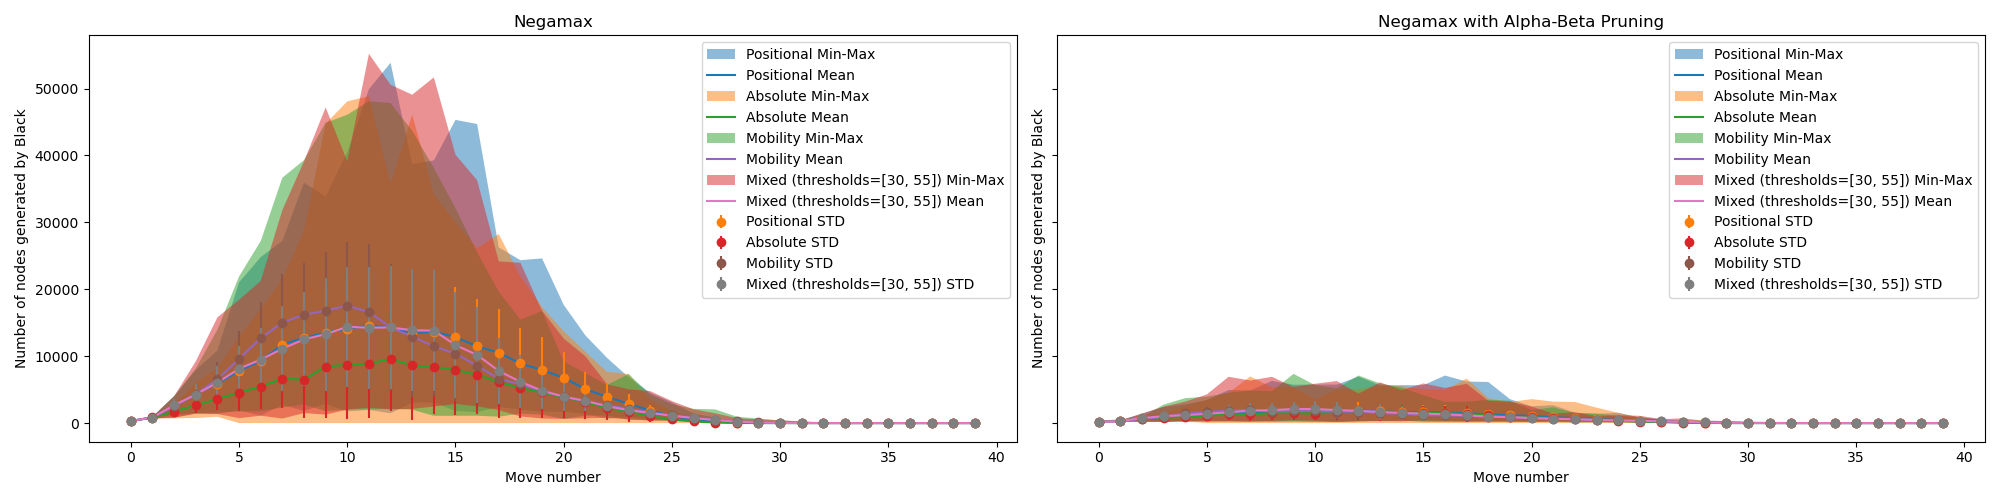
\includegraphics[width=\textwidth]{ressources/Number of nodes generated by Black_depth_4_combined.png}
    \caption{Nombre de nœuds explorés par Minimax et Alpha-Beta en profondeur 4.}
    \label{fig:complexity_node_explored-4}
\end{figure}

\begin{figure}[H]
    \centering
    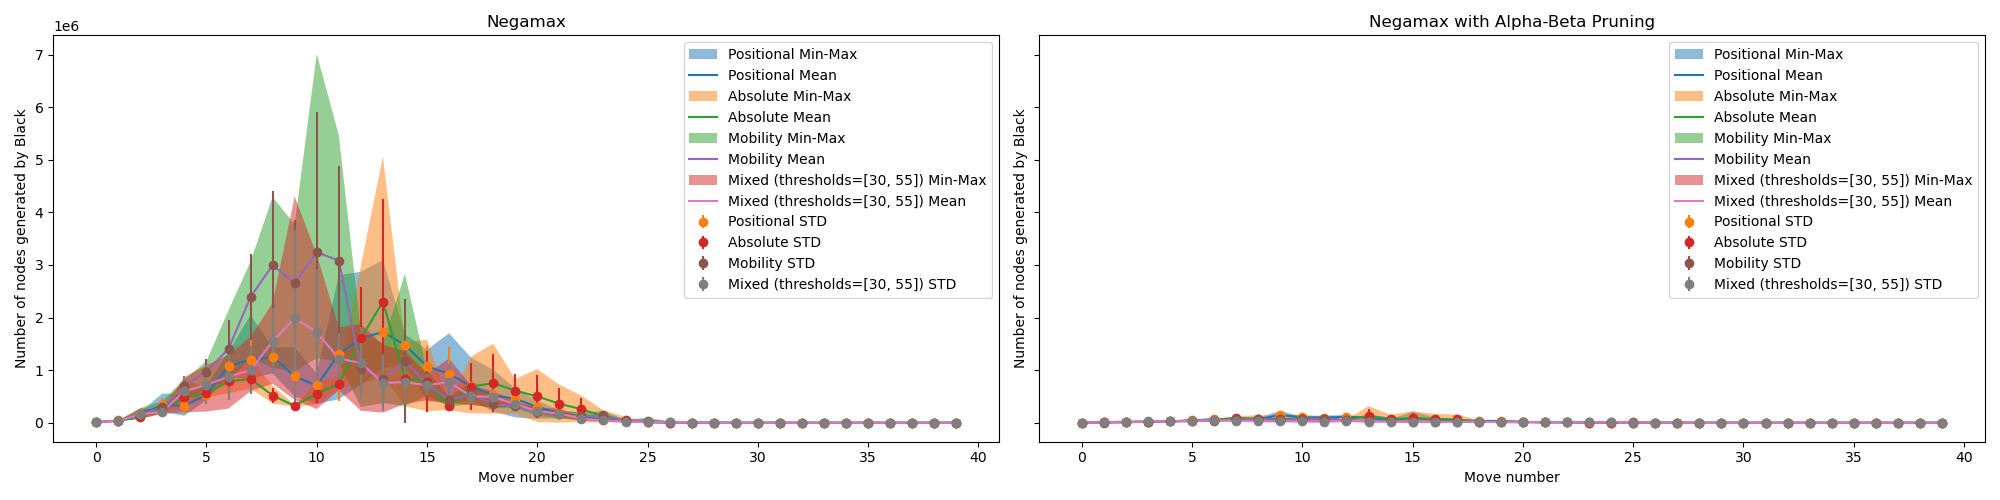
\includegraphics[width=\textwidth]{ressources/Number of nodes generated by Black_depth_6_combined.png}
    \caption{Nombre de nœuds explorés par Minimax et Alpha-Beta en profondeur 6.}
    \label{fig:complexity_node_explored-6}
\end{figure}

Formulons un récapitulatif, nous pouvons observer le nombre moyen de nœuds explorés par Minimax et Alpha-Beta pour chaque profondeur. Les résultats sont présentés dans le tableau \ref{tab:node_explored_summary}. Pour les valeurs exactes, voir le tableau \ref{tab:node_explored_summary-2}, avec pour unité $10^4$ le nombre de nœuds explorés.

\begin{table}[H]
    \centering
    \caption{Analyse comparative du nombre de nœuds explorés en fonction les profondeurs et les stratégies en pourcentage (rapport NegamaxAlphaBeta/Negamax)}
    \resizebox{\textwidth}{!}{% Resize table to fit within the text width, keeping aspect ratio
        \begin{tabular}{
            @{}
            >{\raggedright\arraybackslash}p{1cm}
            >{\raggedright\arraybackslash}p{4cm}
            S
            S
            S
            @{}
            }
            \toprule
            \textbf{Depth} & \textbf{Strategy}           & {\textbf{Max (\%)}} & {\textbf{Mean (\%)}} & {\textbf{Std (\%)}} \\
            \midrule
            \midrule
            \multirow{4}{*}{2}
                           & Positional                  & 58.80               & 57.52                & 65.20               \\
                           & Absolute                    & 64.90               & 55.79                & 63.92               \\
                           & Mobility                    & 54.04               & 53.95                & 60.26               \\
                           & Mixed (thresholds=[30, 55]) & 61.09               & 58.35                & 62.72               \\
            \midrule
            \multirow{4}{*}{4}
                           & Positional                  & 13.19               & 14.77                & 16.35               \\
                           & Absolute                    & 14.27               & 21.19                & 17.92               \\
                           & Mobility                    & 15.29               & 14.06                & 14.30               \\
                           & Mixed (thresholds=[30, 55]) & 12.54               & 15.76                & 15.56               \\
            \midrule
            \multirow{4}{*}{6}
                           & Positional                  & 7.15                & 6.96                 & 6.66                \\
                           & Absolute                    & 6.26                & 7.67                 & 10.21               \\
                           & Mobility                    & 1.93                & 2.98                 & 2.56                \\
                           & Mixed (thresholds=[30, 55]) & 1.84                & 3.07                 & 2.77                \\
            \bottomrule
        \end{tabular}
    }
    \label{tab:node_explored_summary}
\end{table}

\begin{table}[H]
    \centering
    \caption{Analyse comparative du nombre de nœuds explorés en fonction des profondeurs et stratégies (NegamaxAlphaBeta (gauche) vs Negamax(droite))}
    \resizebox{\textwidth}{!}{% Resize table to fit within the text width, keeping aspect ratio
        \begin{tabular}{
            @{}
            >{\raggedright\arraybackslash}p{1cm}
            >{\raggedright\arraybackslash}p{4cm}
            S
            S
            S
            @{}
            }
            \toprule
            \textbf{Depth} & \textbf{Strategy}           & {\textbf{Max $(10^4)$}} & {\textbf{Mean $(10^4)$}} & {\textbf{Std $(10^4)$}} \\
            \midrule
            \midrule
            \multirow{4}{*}{2}
                           & Positional                  & {0.0137 vs 0.0233}      & {0.003193 vs 0.005551}   & {0.001091 vs 0.001673}  \\
                           & Absolute                    & {0.0159 vs 0.0245}      & {0.002579 vs 0.004622}   & {0.001411 vs 0.002208}  \\
                           & Mobility                    & {0.0147 vs 0.0272}      & {0.003256 vs 0.006036}   & {0.001102 vs 0.001830}  \\
                           & Mixed (thresholds=[30, 55]) & {0.0146 vs 0.0239}      & {0.003178 vs 0.005445}   & {0.001087 vs 0.001734}  \\
            \midrule
            \multirow{4}{*}{4}
                           & Positional                  & {0.7103 vs 5.3861}      & {0.078708 vs 0.532977}   & {0.046724 vs 0.285685}  \\
                           & Absolute                    & {0.6975 vs 4.8871}      & {0.068316 vs 0.3224}     & {0.046545 vs 0.259710}  \\
                           & Mobility                    & {0.7352 vs 4.8096}      & {0.073940 vs 0.525755}   & {0.040591 vs 0.283905}  \\
                           & Mixed (thresholds=[30, 55]) & {0.6921 vs 5.5201}      & {0.077103 vs 0.489311}   & {0.044621 vs 0.286737}  \\
            \midrule
            \multirow{4}{*}{6}
                           & Positional                  & {22.08 vs 309.04}       & {2.96 vs 42.50}          & {1.13 vs 16.93}         \\
                           & Absolute                    & {31.68 vs 506.37}       & {2.77 vs 36.06}          & {1.98 vs 19.34}         \\
                           & Mobility                    & {13.56 vs 701.55}       & {1.79 vs 60.19}          & {0.779 vs 30.44}        \\
                           & Mixed (thresholds=[30, 55]) & {7.90 vs 430.26}        & {1.24 vs 40.39}          & {0.582 vs 20.99}        \\
            \bottomrule
        \end{tabular}
    }
    \label{tab:node_explored_summary-2}
\end{table}



\section{Championnat : Comparaison des algorithmes}
\label{sec:championship}

Dans premier temps, comparons les scores en fonctions de l'heuristique utilisée. Les tableaux correspondent à ceux donnés dans le cours. Les scores sont tous simplement le nombre de points obtenues en moyenne par chaque joueur. Nous avons mesuré les scores pour chaque configuration, et les résultats sont présentés dans les tableaux \ref{tab:championship-black} (\ac{PdV} du Joueur Noir) et \ref{tab:championship-white} (\ac{PdV} du Joueur Blanc).

\begin{table}[H]
    \centering
    \caption{Analyse comparative des scores pour le joueur noir en fonction des profondeurs et stratégies (rapport Table d'heuristique 2 (gauche) / Table d'heuristique 1 (droite) et valeurs exactes entre parenthèses)}
    \begin{tabular}{
        @{}
        >{\raggedright\arraybackslash}p{1cm}
        >{\raggedright\arraybackslash}p{4cm}
        S
        S
        @{}
        }
        \toprule
        \textbf{Depth} & \textbf{Strategy}           & {\textbf{Mean (\%)}}      & {\textbf{Std (\%)}}       \\
        \midrule
        \midrule
        \multirow{4}{*}{2}
                       & Positional                  & {119.81 (40.34 vs 33.67)} & {74.22 (8.31 vs 11.20)}   \\
                       & Mixed (thresholds=[30, 55]) & {111.36 (31.26 vs 28.07)} & {118.48 (10.94 vs 9.23)}  \\
        \midrule
        \multirow{4}{*}{4}
                       & Positional                  & {123.77 (39.84 vs 32.19)} & {99.24 (9.33 vs 9.40)}    \\
                       & Mixed (thresholds=[30, 55]) & {102.79 (33.56 vs 32.65)} & {119.15 (11.94 vs 10.02)} \\
        \midrule
        \multirow{4}{*}{6}
                       & Positional                  & {146.67 (39.60 vs 27.00)} & {53.31 (6.41 vs 12.02)}   \\
                       & Mixed (thresholds=[30, 55]) & {116.36 (38.40 vs 33.00)} & {185.24 (12.56 vs 6.78)}  \\
        \bottomrule
    \end{tabular}
    \label{tab:championship-black}
\end{table}

\begin{table}[H]
    \centering
    \caption{Analyse comparative des scores pour le joueur blanc en fonction des profondeurs et stratégies (rapport Table d'heuristique 2 (gauche) / Table d'heuristique 1 (droite) et valeurs exactes entre parenthèses)}
    \begin{tabular}{
        @{}
        >{\raggedright\arraybackslash}p{1cm}
        >{\raggedright\arraybackslash}p{4cm}
        S
        S
        @{}
        }
        \toprule
        \textbf{Depth} & \textbf{Strategy}           & {\textbf{Mean (\%)}}      & {\textbf{Std (\%)}}      \\
        \midrule
        \midrule
        \multirow{4}{*}{2}
                       & Positional                  & {128.22 (38.85 vs 30.30)} & {83.51 (9.34 vs 11.19)}  \\
                       & Mixed (thresholds=[30, 55]) & {110.02 (31.28 vs 28.43)} & {115.42 (10.44 vs 9.05)} \\
        \midrule
        \multirow{4}{*}{4}
                       & Positional                  & {97.70 (31.06 vs 31.79)}  & {199.38 (18.76 vs 9.41)} \\
                       & Mixed (thresholds=[30, 55]) & {90.55 (29.52 vs 32.60)}  & {218.67 (18.74 vs 8.57)} \\
        \midrule
        \multirow{4}{*}{6}
                       & Positional                  & {114.05 (42.20 vs 37.00)} & {76.89 (9.24 vs 12.02)}  \\
                       & Mixed (thresholds=[30, 55]) & {136.42 (47.20 vs 34.60)} & {140.46 (12.98 vs 9.24)} \\
        \bottomrule
    \end{tabular}
    \label{tab:championship-white}
\end{table}

Nous voulons maintenant comparer les statégies et l'aventage potentielle d'une couleur sur l'autre. Les résultats sont présentés dans les tableaux \ref{tab:championship-overall-black} et \ref{tab:championship-overall-white}.

\begin{table}[H]
    \centering
    \caption{Analyse comparative des scores en fonction des profondeurs et stratégies pour toutes les configurations du Joueur Noir}
    \begin{tabular}{
        @{}
        >{\raggedright\arraybackslash}p{1cm}
        >{\raggedright\arraybackslash}p{4cm}
        S
        S
        S
        S
        @{}
        }
        \toprule
        \textbf{Depth} & \textbf{Strategy}           & \textbf{Min} & \textbf{Max} & \textbf{Mean} & \textbf{STD} \\
        \midrule
        \midrule
        \multirow{4}{*}{2}
                       & Positional                  & 0            & 58           & 35.458        & 9.625        \\
                       & Absolute                    & 0            & 62           & 24.293        & 10.102       \\
                       & Mobility                    & 0            & 62           & 26.970        & 12.160       \\
                       & Mixed (thresholds=[30, 55]) & 0            & 62           & 34.087        & 10.988       \\
        \midrule
        \multirow{4}{*}{4}
                       & Positional                  & 0            & 59           & 32.700        & 9.036        \\
                       & Absolute                    & 0            & 61           & 22.435        & 10.036       \\
                       & Mobility                    & 0            & 63           & 30.713        & 11.977       \\
                       & Mixed (thresholds=[30, 55]) & 0            & 64           & 34.940        & 11.650       \\
        \midrule
        \multirow{4}{*}{6}
                       & Positional                  & 0            & 52           & 29.567        & 10.607       \\
                       & Absolute                    & 2            & 59           & 26.330        & 8.536        \\
                       & Mobility                    & 0            & 61           & 30.348        & 12.611       \\
                       & Mixed (thresholds=[30, 55]) & 11           & 63           & 37.983        & 9.909        \\
        \bottomrule
    \end{tabular}
    \label{tab:championship-overall-black}
\end{table}

\begin{table}[H]
    \centering
    \caption{Analyse comparative des scores en fonction des profondeurs et stratégies pour toutes les configurations du Joueur Blanc}
    \begin{tabular}{
        @{}
        >{\raggedright\arraybackslash}p{1cm}
        >{\raggedright\arraybackslash}p{4cm}
        S
        S
        S
        S
        @{}
        }
        \toprule
        \textbf{Depth} & \textbf{Strategy}           & \textbf{Min} & \textbf{Max} & \textbf{Mean} & \textbf{STD} \\
        \midrule
        \multirow{4}{*}{2}
                       & Positional                  & 0            & 58           & 34.953        & 9.872        \\
                       & Absolute                    & 0            & 58           & 24.765        & 9.955        \\
                       & Mobility                    & 0            & 62           & 29.325        & 11.069       \\
                       & Mixed (thresholds=[30, 55]) & 0            & 62           & 33.524        & 11.563       \\
        \midrule
        \multirow{4}{*}{4}
                       & Positional                  & 0            & 57           & 31.909        & 11.554       \\
                       & Absolute                    & 0            & 63           & 23.343        & 10.259       \\
                       & Mobility                    & 0            & 64           & 27.855        & 11.188       \\
                       & Mixed (thresholds=[30, 55]) & 0            & 62           & 34.292        & 12.563       \\
        \midrule
        \multirow{4}{*}{6}
                       & Positional                  & 7            & 59           & 32.967        & 8.770        \\
                       & Absolute                    & 0            & 58           & 21.987        & 12.139       \\
                       & Mobility                    & 0            & 60           & 29.556        & 11.584       \\
                       & Mixed (thresholds=[30, 55]) & 0            & 60           & 34.700        & 11.150       \\
        \bottomrule
    \end{tabular}
    \label{tab:championship-overall-white}
\end{table}

